A continuación se presentan los resultados obtenidos del modelo cnn\_base\_tt detallados en la figura \ref{fig:exactitud}, donde se observa que el modelo sufre de sobreajuste, ya que la precisión en el conjunto de entrenamiento aumenta constantemente a medida que avanzan las épocas, mientras que la precisión en el conjunto de validación disminuye.

\begin{figure}[h!]
	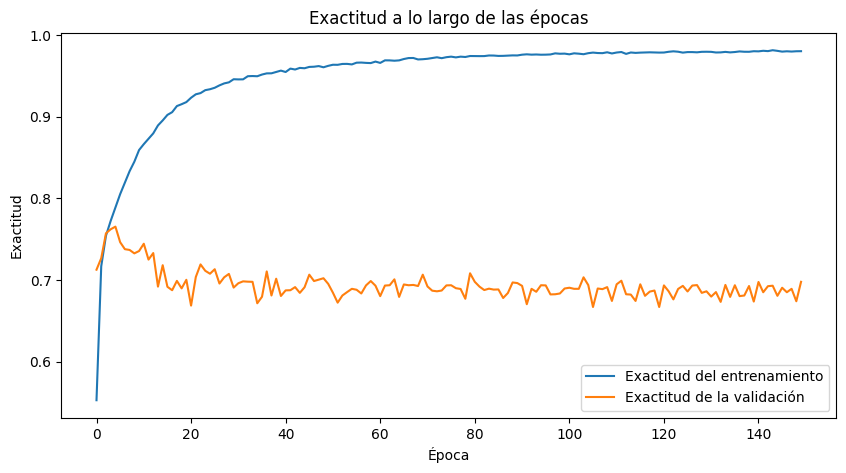
\includegraphics[width=0.65\textwidth]{capitulo5/figuras/exactitud.png}
	\caption{Exactitud del modelo base
		\\\textit{Fuente: Elaboracion Propia}}
	\label{fig:exactitud}
\end{figure}

 De igual forma en la figura \ref{fig:perdida}, se muestra que el error en el conjunto de validación crece con el tiempo, mientras que el error en el conjunto de entrenamiento disminuye, los resultados específicos obtenidos bajo las métricas seleccionadas se presentan en la tabla \ref{tbl:6}. Todos estos resultados obtenidos por el modelo cnn\_base\_tt  sugieren la necesidad de utilizar técnicas de regularización para mitigar el sobreajuste.



\begin{figure}[h!]
	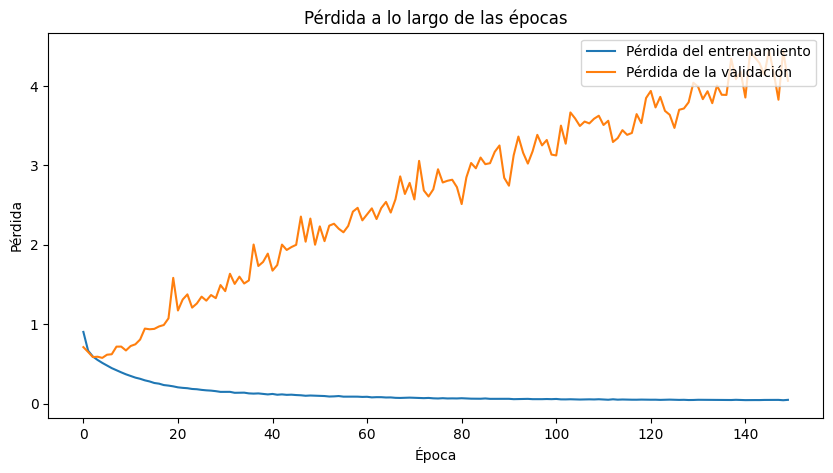
\includegraphics[width=0.65\textwidth]{capitulo5/figuras/perdida.png}
	\caption{Perdida del modelo base
		\\\textit{Fuente: Elaboracion Propia}}
	\label{fig:perdida}
\end{figure}

\begin{table}[!ht]
	\centering
	\begin{tabular}{|c|c|c|c|c|c|}
		\hline
		\textbf{Nombre del modelo} & \textbf{Precisión} & \textbf{Perdida} & \textbf{Val\_Precisión} & \textbf{Val\_Perdida} & \textbf{Epoca} \\ \hline
		~ & 0.7522 & 0.59 & 0.7650 & 0.5743 & 3 \\ \cline{2-6} 
		cnn\_base\_tt & 0.978 & 0.04 & 0.7128 & 3.3866 & 109 \\ \cline{2-6} 
		~ & 0.9811 & 0.04 & 0.6893 & 3.8825 & 150 \\ \hline
	\end{tabular}
	\caption{Detalle resultados del modelo cnn\_base\_tt
		\\\textit{Fuente: Elaboracion Propia}}
	\label{tbl:6}
\end{table}

Debido al sobreajuste demostrado en los resultados del modelo cnn\_base\_tt se utilizaron técnicas de regularización con nuevos modelos, Los resultados obtenidos de cada uno de estos modelos regularizados se presentan en la tabla \ref{tbl:7}.

\begin{table}[!ht]
	\centering
	\begin{tabular}{|c|c|c|c|c|c|}
		\hline
		\textbf{Nombre del modelo} & \textbf{Precisión} & \textbf{Perdida} & \textbf{Val\_Precisión} & \textbf{Val\_Perdida} & \textbf{Epoca} \\ \hline
		~ & 0.7890 & 0.52 & 0.7341 & 0.6090 & 4 \\ \cline{2-6} 
		cnn\_base\_bn\_tt & 0.9757 & 0.05 & 0.7272 & 2.8434 & 91 \\ \cline{2-6} 
		~ & 0.9800 & 0.04 & 0.5783 & 3.0617 & 150 \\ \hline
		~ & 0.7752 & 0.56 & 0.7646 & 0.5670 & 7 \\ \cline{2-6} 
		cnn\_base\_dp\_tt & 0.9000 & 0.25 & 0.7400 & 0.9013 & 133 \\ \cline{2-6} 
		~ & 0.9038 & 0.24 & 0.7274 & 0.8862 & 150 \\ \hline
		~ & 0.4185 & 1.02 & 0.4048 & 1.0484 & 123 \\ \cline{2-6} 
		cnn\_base\_l2\_tt & 0.4191 & 1.02 & 0.4048 & 1.0500 & 128 \\ \cline{2-6} 
		~ & 0.4118 & 1.02 & 0.4048 & 1.0503 & 150 \\ \hline
	\end{tabular}
	\caption{Resultados de modelos regularizados
		\\\textit{Fuente: Elaboracion Propia}}
	\label{tbl:7}
\end{table}

En los resultados detallados en la tabla \ref{tbl:7}, se observa que los métodos de regularización dropout y batch normalization (BN) retrasaron el sobreajuste. Sin embargo, al considerar el mejor modelo guardado con el menor error, el resultado es casi similar al obtenido por el modelo no regularizado. Por lo tanto, se probó el uso de dos técnicas de regularización simultáneamente en los modelos. A continuación se detallan los resultados obtenidos en los modelos que usan dos técnicas de regularización:

\begin{table}[!ht]
	\centering
	\begin{tabular}{|c|c|c|c|c|c|}
		\hline
		\textbf{Nombre del modelo} & \textbf{Precisión} & \textbf{Perdida} & \textbf{Val\_Precisión} & \textbf{Val\_Perdida} & \textbf{Epoca} \\ \hline
		~ & 0.8135 & 0.47 & 0.7596 & 0.5652 & 22 \\ \cline{2-6}
		cnn\_base\_bndp\_128t & 0.8967 & 0.26 & 0.7463 & 0.7757 & 126 \\ \cline{2-6}
		~ & 0.9029 & 0.25 & 0.7204 & 0.8861 & 150 \\ \hline
		~ & 0.7738 & 0.56 & 0.7777 & 0.5373 & 12 \\ \cline{2-6}
		cnn\_base\_bndp\_64t & 0.8701 & 0.34 & 0.7621 & 0.6211 & 65 \\ \cline{2-6}
		~ & 0.9058 & 0.25 & 0.7531 & 0.7155 & 150 \\ \hline
		~ & 0.8084 & 0.48 & 0.7804 & 0.5584 & 26 \\ \cline{2-6}
		cnn\_base\_bndp\_32t & 0.8580 & 0.37 & 0.7627 & 0.6342 & 56 \\ \cline{2-6}
		~ & 0.8962 & 0.28 & 0.7436 & 0.7562 & 150 \\ \hline
	\end{tabular}
	\caption{Resultados de modelos regularizados
		\\\textit{Fuente: Elaboracion Propia}}
	\label{tbl:8}
\end{table}

Los resultados obtenidos en la tabla algo \ref{tbl:8} demuestran que, sin importar la época, el error en el conjunto de validación no sobrepasará el valor de 1.0 y siempre se mantendrá por debajo de ese rango. La precisión en el conjunto de validación se mantendrá siempre por encima de 0.75 en la época con menor perdida de cada modelo, siendo la mejor métrica de 0.78 obtenida por el modelo cnn\_base\_bndp\_32t, mismo que supera en 2 puntos la precisión del modelo base. Sin embargo, el modelo cnn\_base\_bndp\_64t es el que obtiene la menor pérdida.


